\documentclass[11pt]{article}
\usepackage[italian]{babel}
\usepackage{geometry}
\usepackage{pifont}
\usepackage{graphicx} 
\usepackage{subcaption}
\usepackage{titlesec}
\usepackage{wrapfig}
\geometry{a4paper} 
\usepackage{listings} % necessario per inclusione codice sorgente
\usepackage{color} % syntax highlighting
\usepackage{url}
\usepackage[export]{adjustbox}
% definizione dei colori  
\definecolor{dkgreen}{rgb}{0,0.6,0}
\definecolor{gray}{rgb}{0.5,0.5,0.5}
\definecolor{mauve}{rgb}{0.58,0,0.82}

\pdfinfo{
   /Author (Andrei Ciulpan)
   /Title  (Guitar Hero in Logisim - Relazione del Progetto di Laboratorio - Architetture I - Turno A)
}
\title{Relazione del progetto di Architetture I\\ Guitar Hero in Logisim\thanks{Progetto approvato il 20/08/2018 e consegnato il 23/08/2018}}
\author{Andrei Ciulpan\\ Matricola: 872394 - Turno: A\\ \url{andrei.ciulpan@studenti.unimi.it}}
\date{}

\begin{document}
\maketitle

\section{Introduzione}

\begin{figure}[!htpb]
\centering
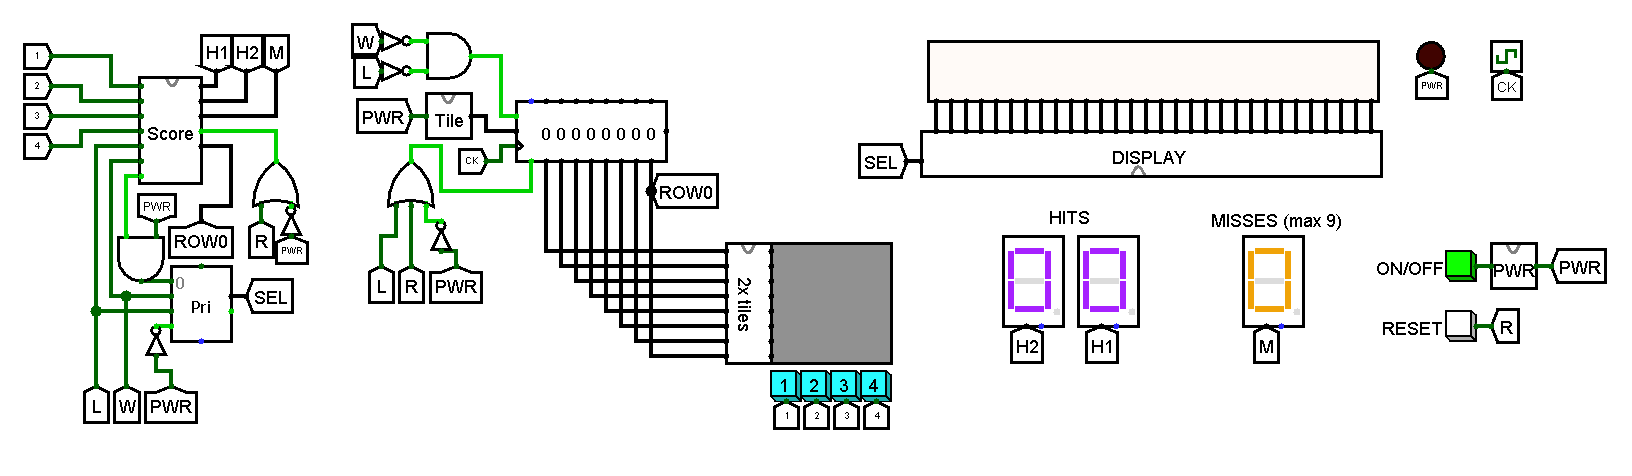
\includegraphics[width=1.3\textwidth, center]{immagini/main}
\caption{User interface completa}
\label{fig:fig1}
\end{figure}

Il progetto consiste nel simulare il gioco "Guitar Hero" in cui un giocatore ha il compito di premere dei bottoni
nel momento opportuno per guadagnare dei punti. Per momento opportuno intendo il momento in cui i "tiles" 
arrivano in fondo della schermata di gioco.
\\Per presentare il progetto ho deciso di seguire un approccio top-down in cui parto dalla figura in  cui esso viene
rappresentato nella sua interezza  (Figura 1)  per poi continuare descrivendo le varie parti che lo compongono.

\pagebreak
\section{Board di Gioco}

\begin{figure}[!htpb]
\centering
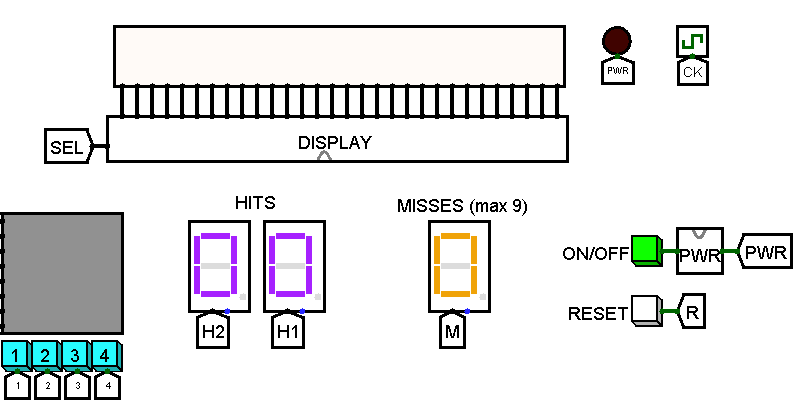
\includegraphics[width=1\textwidth, center]{immagini/board_di_gioco_completa}
\caption{Board di gioco}
\label{fig:fig2}
\end{figure}

La board di gioco è rappresentata da:
\begin{enumerate}
\item una matrice LED 8x8 per visualizzare i "tiles"
\item una matrice LED 4x30 per visualizzare i messaggi di "YOU WON" oppure "YOU LOST" a fine partita
\item due HEX digit display per il conteggio dei punti (max 20) e un HEX digit display per il conteggio degli errori (max 9)
\item bottone di ON/OFF
\item bottone di RESET
\item 4 bottoni usati per il gameplay
\end{enumerate}

Ogni componente enumerato verrà trattato nel dettaglio nelle seguenti sottosezioni.
\pagebreak
\subsection{Matrice LED 8x8 e l'effetto dei "tiles" cadenti}

\begin{figure}[!htpb]
\centering
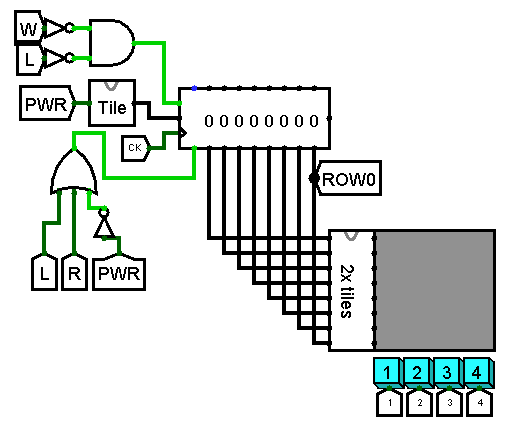
\includegraphics[width=0.8\textwidth, center]{immagini/gestione_tile}
\caption{Gestione della schermata di gioco}
\label{fig:fig3}
\end{figure}

La matrice LED 8x8 è pilotata da un shift register a 8 stadi (una per ogni riga della matrice).
Il shift register riceve in ingresso un numero pseudo-random su 4 bit dal componente chiamato "Tile".
Questo numero su 4 bit, appena entrato nel shift register, accenderà (o non), dopo aver passato nel circuito "Tile doubler", 
due celle adiacenti dell'ultima riga della matrice LED (questa scelta è stata fatta per poter avere una matrice piu' grande
e quindi per poter allineare bene i bottoni con le colonne della matrice). Al colpo di clock successivo questo numero è shiftato a destra e
 accenderà quindi le due celle adiacenti della riga sottostante dando l'effetto dei "tiles" cadenti.
\\Nei paragrafi successivi descriverò il modo in cui i "tiles" vengono raddoppiati e come vengono generati questi numeri casuali all'interno del componente "Tile".

\pagebreak
\subsubsection{Circuito che raddoppia i "tiles"}

\begin{figure}[h]
\begin{subfigure}{0.3\textwidth}
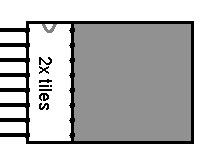
\includegraphics[width=0.95\linewidth, height=5cm]{immagini/componente_tile_doubler} 
\caption{Il componente che raddoppia i "tiles"}
\label{fig:subfig8}
\end{subfigure}
\begin{subfigure}{0.7\textwidth}
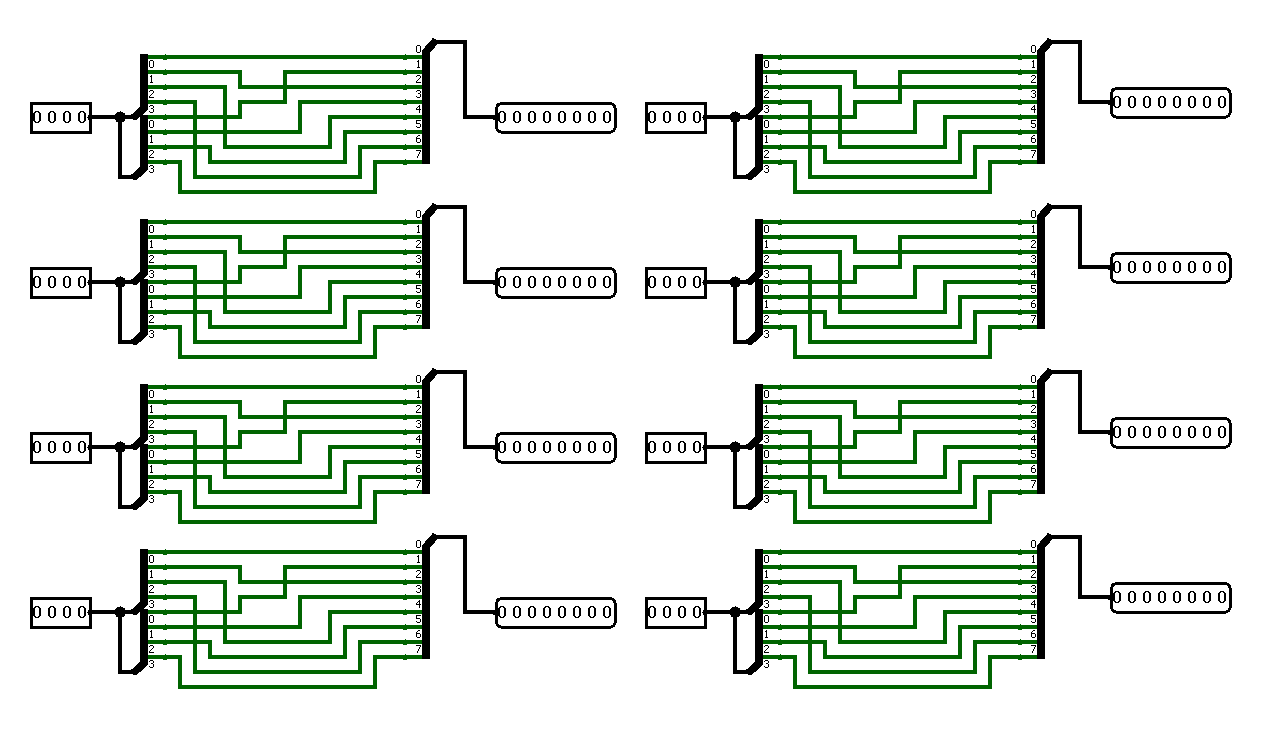
\includegraphics[width=1.1\linewidth, height=5cm]{immagini/circuito_tile_doubler}
\caption{Circuito che conta i punti}
\label{fig:subfig10}
\end{subfigure}
\caption{Circuito del componente che raddoppia i "tiles"}
\label{fig:fig15}
\end{figure}

Questo componente riceve all'ingresso un numero su 4 bit e da in uscita un numero su 8 bit
dopo aver raggruppato due bit adiacenti alla volta in modo che abbiano lo stesso valore. Questo lavoro
è svolto grazie al modo in cui si possono collegare i bit dei vari splitter tra di loro.
Siccome il nostro circuito può ricevere in ingresso soltanto un valore tra 0, 1, 2, 4 e 8 alla volta (grazie al circuito "Tile Generator"),
mi limiterò a scrivere le uscite solo per questi valori:

\begin{itemize}
\item 1000 \ding{212} 1100 0000
\item 0100 \ding{212} 0011 0000
\item 0010 \ding{212} 0000 1100
\item 0001 \ding{212} 0000 0011
\item 0000 \ding{212} 0000 0000
\end{itemize}

Guardando le uscite del nostro componente possiamo notare che nella nostra matrice LED ci saranno sempre 2 pixel adiacenti accesi (o spenti).
\pagebreak
\subsubsection{Circuito per la generazione casuale dei "tiles"}

\begin{figure}[!htpb]
\centering
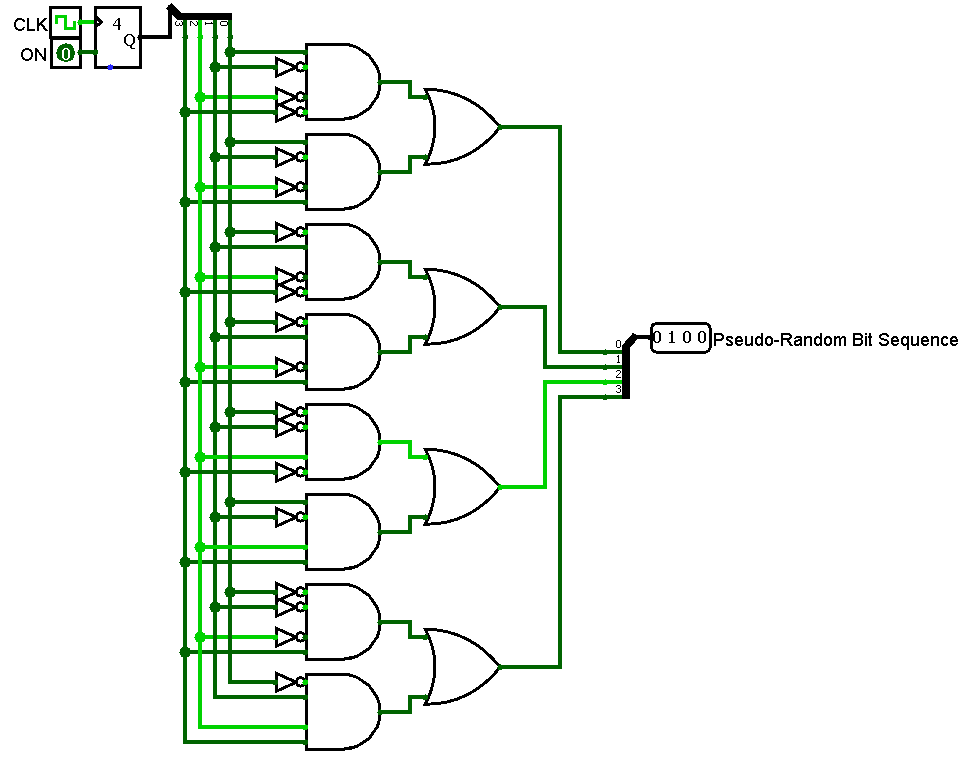
\includegraphics[width=0.7\textwidth, center]{immagini/circuito_tiles}
\caption{Circuito per la generazione casuale dei "tiles"}
\label{fig:fig4}
\end{figure}

Nella figura 4 si può notare un componente che si chiama Random Generator. Esso è impostato
per generare un numero pseudo-random su 4 bit che poi entrerà (dopo alcune modifiche) nello shift 
register che pilota la matrice LED.
Il generatore dei numeri random, essendo su 4 bit, genera un numero da 0 a 15 ad ogni colpo di clock.
Questo numero viene poi dato ad un circuito SOP che attiva una (o nessuna) delle 4 linee in uscita (queste
4 linee rappresentano le colonne della matrice LED e al piu' una linea può essere accesa alla volta). 
\\
\\Particolarmente:
\begin{itemize}
\item la linea 0 viene attivata quando il numero generato è 1 oppure 9
\item la linea 1 viene attivata quando il numero generato è 2 oppure 10
\item la linea 2 viene attivata quando il numero generato è 4 oppure 13
\item la linea 3 viene attivata quando il numero generato è 8 oppure 14
\item in tutti gli altri casi le linee sono messe a 0 e quindi non abbiamo nessun "tile" in quel istante
\end{itemize}
In questo modo ad ogni ciclo di clock c'è una probabilità  di 50\% di trovare un tile, dopo aver raddoppiato i pixel, su esattamente due delle otto colonne.

\subsection{Matrice LED 4x30 e la visualizzazione dei messaggi a fine partita}

\begin{figure}[!htpb]
\centering
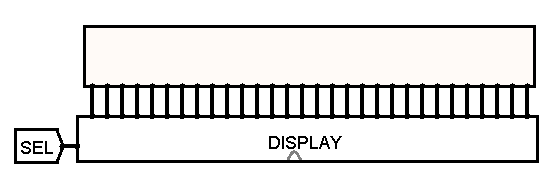
\includegraphics[width=0.7\textwidth, center]{immagini/matrice_led4x30}
\caption{Matrice LED 4x30}
\label{fig:fig5}
\end{figure}

Su questa matrice LED, pilotata dal componente "DISPLAY", si possono visualizzare  i seguenti messaggi:
\begin{itemize}
\item "YOU WON" dopo aver guadagnato 20 punti
\item "YOU LOST" dopo aver sbagliato 9 volte
\item "PLAY" durante il gameplay
\end{itemize}

\subsubsection{Circuito per visualizzare i messaggi}

\begin{figure}[!htpb]
\centering
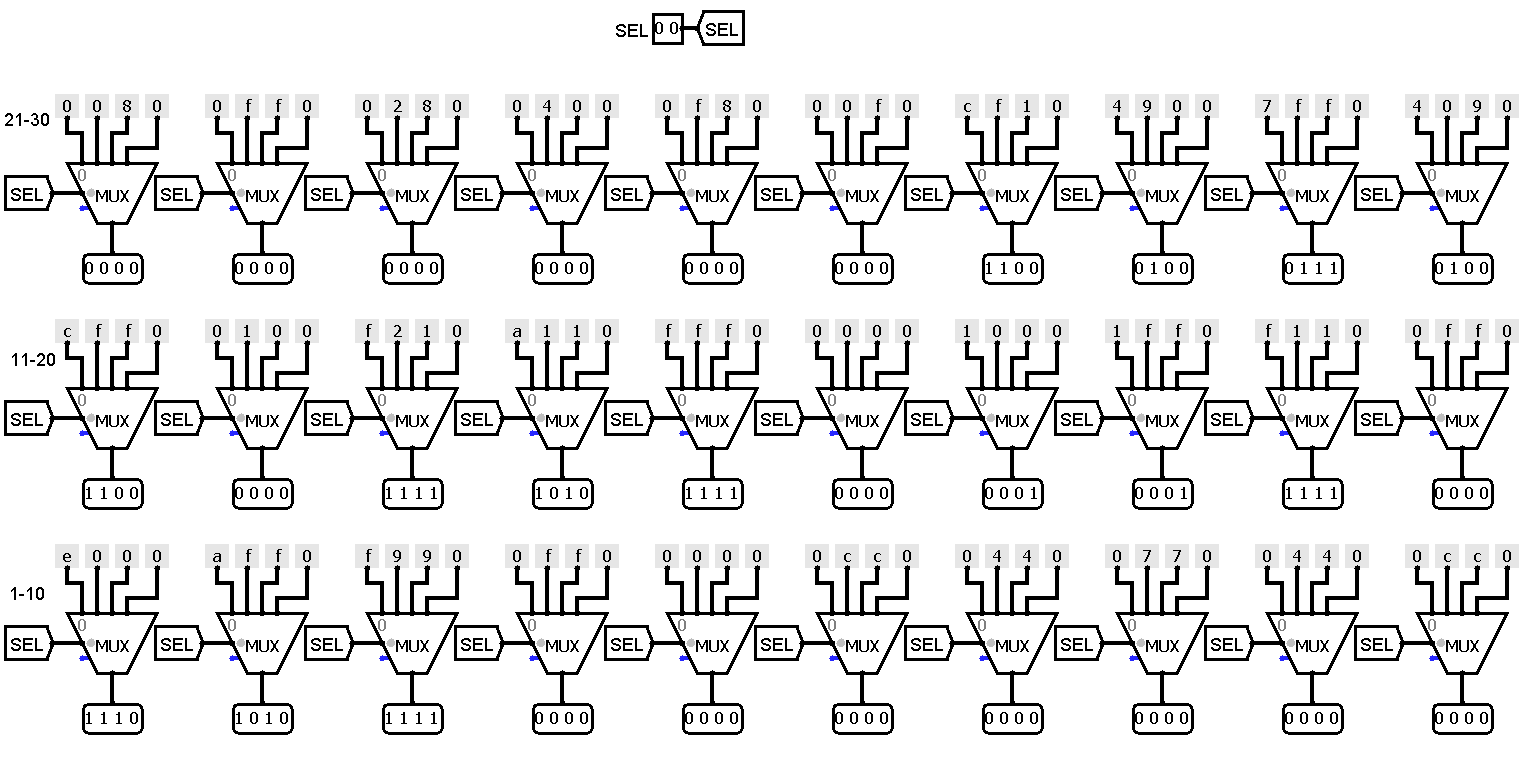
\includegraphics[width=1.15\textwidth, center]{immagini/circuito_matriceLED4x30}
\caption{Circuito per la generazione dei messaggi}
\label{fig:fig6}
\end{figure}

La matrice LED 4x30 è indirizzata per colonna, perciò bisogna indirizzare 30 colonne.
Ogni elemento nella figura 6 indirizza una sola colonna della matrice. Mandando dei segnali
costanti opportuni possiamo accendere solo alcune righe di ciascuna colonna e quindi scrivere
qualsiasi lettera. Ogni colonna può essere indirizzata da 4 valori diversi (ciò è scelto dal MUX a 2 vie), 
tramite il segnale di selezione SEL a 2 bit, a seconda delle necessità:
\begin{itemize}
\item SEL = 00 \ding{212} "PLAY" 
\item SEL = 01 \ding{212} "YOU WON"
\item SEL = 10 \ding{212} "YOU LOST"
\item SEL = 11 \ding{212} Matrice LED spenta (il circuito è spento)
\end{itemize}

\begin{wrapfigure}{l}{0.5\textwidth}
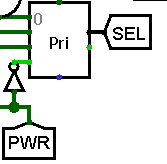
\includegraphics[width=0.9\linewidth]{immagini/encoder} 
\caption{Encoder}
\label{fig:fig7}
\end{wrapfigure}

Il segnale di selezione viene ricevuto da un encoder (che si può vedere in figura 7).
L'encoder manderà in uscita una sequenza su 2 bit in base a quale linea è accesa al suo ingresso:

\begin{itemize}
\item SEL = 00 \ding{212} la prima linea è accesa (l'uscita "IN PROGRESS" del componente che calcola lo score messa in AND con la linea ON/OFF)
\item SEL = 01 \ding{212} la seconda linea è accesa (l'uscita "WIN" del componente che calcola lo score)
\item SEL = 10 \ding{212} la terza linea è accesa (l'uscita "LOSE" del componente che calcola lo score)
\item SEL = 11 \ding{212} la quarta linea è accesa (l'uscita negata della linea di ON/OFF)
\end{itemize}

\pagebreak
\subsection{Conteggio dei punti e degli errori}

\begin{figure}[!htpb]
\centering
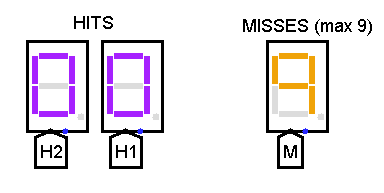
\includegraphics[width=0.6\textwidth, center]{immagini/hex_digit_display}
\caption{Tre HEX digit display}
\label{fig:fig8}
\end{figure}

In questa fase utilizziamo i tre HEX digit display (due per i punti, uno per gli errori)
\subsubsection{Conteggio dei punti}

\begin{figure}[h]
\begin{subfigure}{0.3\textwidth}
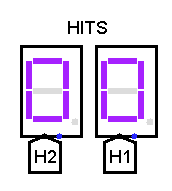
\includegraphics[width=1\linewidth, height=5.5cm]{immagini/hex_digit_display_hit} 
\caption{Due HEX digit display usati per visualizzare i punti}
\label{fig:subfig1}
\end{subfigure}
\begin{subfigure}{0.8\textwidth}
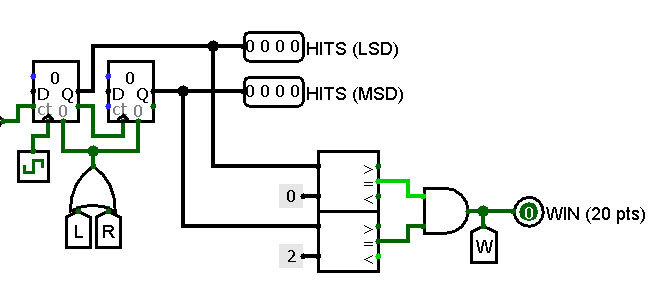
\includegraphics[width=1.05\linewidth, height=5.5cm]{immagini/circuito_hit}
\caption{Circuito che conta i punti}
\label{fig:subfig2}
\end{subfigure}
\caption{Circuito completo per il conteggio dei punti}
\label{fig:fig9}
\end{figure}

Nella figura 9.b) si possono vedere 2 contatori su 4 bit messi in sequenza.
Il primo (quello piu' a sinistra) conta fino a 9 e quando lo supera (il contatore 
sente il clock sul falling edge) alza la linea di carry che poi fa da clock al secondo contatore.
In questo modo il primo contatore torna a 0 dopo aver mandato il carry al secondo contatore
che a sua volta incrementa di 1.
I valori del primo e del secondo contatore vanno poi mandati in uscita come due sequenze
di 4 bit (una che rappresenta le unità $LSD$  e l'altro le decine $MSD$). Ciascuna sequenza
pilota uno dei due display nella figura 9.a).
\\Inoltre l'uscita WIN è pilotata dalle uscite di 2 comparatori messe in AND. I comparatori alzano la loro linea di uscita
quando i due contatori segnano rispettivamente 0 per LSD e 2 per MSD (ovvero quando si arriva a 20).
\\Come detto prima questo segnale di WIN attiva il circuito adatto che pilota il display per poter visualizzare
il messaggio "YOU WON".
\\Il circuito che manda i segnali di HIT che incrementano i contatori è presentato nella sezione 2.6.
\subsubsection{Conteggio degli errori}

\begin{figure}[h]
\begin{subfigure}{0.35\textwidth}
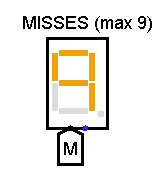
\includegraphics[width=1\linewidth, height=5.5cm]{immagini/hex_digit_display_miss} 
\caption{Un HEX digit display usato per visualizzare gli errori}
\label{fig:subfig3}
\end{subfigure}
\begin{subfigure}{0.6\textwidth}
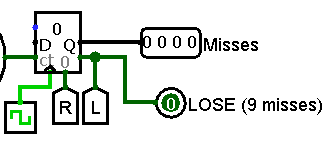
\includegraphics[width=1.05\linewidth, height=5.5cm]{immagini/circuito_miss}
\caption{Circuito che conta gli errori}
\label{fig:subfig4}
\end{subfigure}
\caption{Circuito completo per il conteggio degli errori}
\label{fig:fig10}
\end{figure}

Nella figura 10.b) si può vedere un contatore su 4 bit che è impostato a poter contare solo fino a 9.
Il valore del contatore viene mandato fuori dal circuito come una sequenza di 4 bit che poi entrerà nel display che si può vedere nella figura
10.a).
Quando supera il 9 (il contatore è impostato a sentire il falling edge del clock) esso aumenta la linea di carry che poi sarà il nostro segnale di LOSE.
\\Il circuito che manda i segnali di MISS che incrementano il contatore è presentato nella sezione 2.6.

\pagebreak

\subsection{Circuito di ON/OFF}

\begin{figure}[h]
\begin{subfigure}{0.45\textwidth}
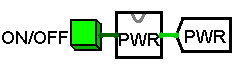
\includegraphics[width=1\linewidth, height=4.5cm]{immagini/on_off} 
\caption{Bottone di accensione/spegnimento del circuito}
\label{fig:subfig5}
\end{subfigure}
\begin{subfigure}{0.45\textwidth}
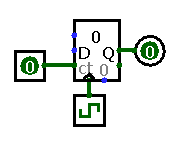
\includegraphics[width=1.2\linewidth, height=4.5cm]{immagini/circuito_on_off}
\caption{Circuito di accensione/spegnimento del circuito}
\label{fig:subfig6}
\end{subfigure}
\caption{Circuito completo per accensione/spegnimento}
\label{fig:fig11}
\end{figure}

Il circuito di accensione/spegnimento nella figura 11.b) è implementato da un contatore su 1 bit
(e quindi che conta solo fino a 1). Quando viene premuto il bottone di ON/OFF nella figura 11.a), durante il
rising edge del clock, il contatore aumenta a 1. Quando il bottone viene premuto di nuovo il contatore è
già in overflow e passa a 0 (grazie all'impostazione di wrap around) e cosi' via.

\subsection{Reset}

\begin{figure}[!htpb]
\centering
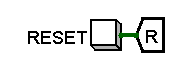
\includegraphics[width=0.4\textwidth, center]{immagini/reset}
\caption{Bottone per il RESET}
\label{fig:fig12}
\end{figure}

Il segnale di RESET fa tornare il gioco allo stato iniziale che si ha subito dopo l'accensione.
Questo viene fatto azzerrando lo stato del shift register e dei contatori.

\pagebreak 

\subsection{I 4 bottoni per il gameplay e l'interazione con lo stato del gioco}

\begin{figure}[h]
\begin{subfigure}{0.4\textwidth}
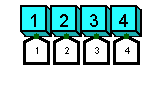
\includegraphics[width=0.8\linewidth, height=4.5cm]{immagini/bottoni} 
\caption{4 bottoni per il gameplay}
\label{fig:subfig7}
\end{subfigure}
\begin{subfigure}{0.5\textwidth}
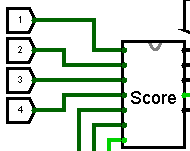
\includegraphics[width=1\linewidth, height=4.5cm]{immagini/input_score}
\caption{Bottoni come input nel circuito che calcola lo score}
\label{fig:subfig8}
\end{subfigure}
\caption{Bottoni e come essi influiscono sullo stato del gioco}
\label{fig:fig13}
\end{figure}

I 4 bottoni rappresentano 4 input per il circuito che calcola lo score.
Inoltre in questo circuito entra anche la sequenza di 4 bit uscente dall'ultimo stadio
dello shift register che, come detto nella sezione 2.1, pilota la prima riga
della matrice LED 8x8 (ROW 0).
Questi 8 bit rappresentano i i nostri input nel circuito score che influiscono
sullo stato della macchina.

\pagebreak
\subsubsection{Interazione degli input con lo stato del gioco}

\begin{figure}[!htpb]
\centering
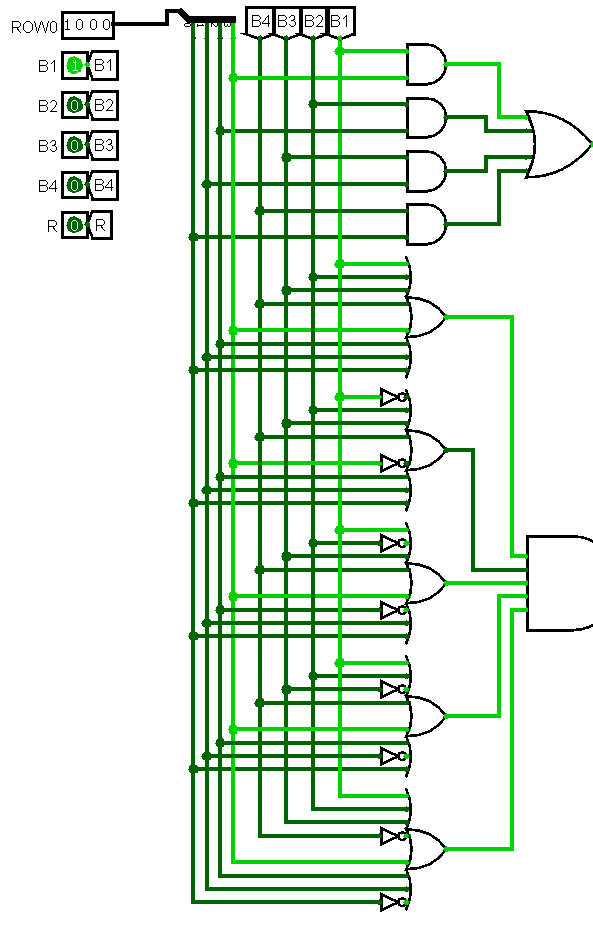
\includegraphics[width=0.8\textwidth, center]{immagini/SOP_POS_score}
\caption{Circuito che fa scattare i contatori dei punti e degli errori}
\label{fig:fig14}
\end{figure}

Nella figura 14 si possono vedere gli 8 input del nostro circuito (tra cui 4 arrivano dai bottoni per il gameplay
e gli altri 4 arrivano dall'ultimo stadio del nostro shift register (ovvero ROW 0).
\\La parte in alto che rappresenta la SOP è utilizzata per pilotare il contatore degli HIT (e.g. che incrementa 
quando il bottone 1 è premuto e contemporaneamente la linea che rappresenta la prima colonna
della riga 0 è accesa).
\\La parte in basso che rappresenta la POS è utilizzata per pilotare il contatore dei MISS (e.g che incrementa quando
è accesa la linea che rappresenta la prima colonna della riga 0 ma il bottone 1 non è stato premuto e quindi la linea B1 è spenta)
\section{Conclusioni}

Per realizzare il circuito sono partito dall'implementazione della board di gioco con il shift registe e la matrice LED, che inizalmente era 8x2. Poi ho
rifatto la stessa cosa su una scala piu' grande (matrice LED 8x8) e infine ho aggiunto lo score e la matrice per visualizzare i messaggi a fine partita.
\\ \\
Miglioramenti possibili:
\begin{itemize}
\item aumentare la scala della board di gioco
\item risolvere un bug derivato dallo stato del gioco dopo aver vinto (il contatore non dovrebbe piu' aumentare)
\item possibilità di selezionare la difficoltà con un circuito che aumenta la probabilità di generare i "tiles".
\end{itemize}
\end{document}
